% !TEXroot=main.tex
\section{Lösungskonzept}
{
	Zur Lösung der Aufgabe wurde ein Turtlebot Roboter benutzt. Dieser ermöglicht durch den Raspberry Pi, welcher eingebaut ist, eine einfache Programmierung. Auf dem Raspberry Pi läuft das Robot-Operating-Systme, was eine einfache Steuerung und Programmierung ermöglicht.
	\begin{figure}[H]
		\centering
		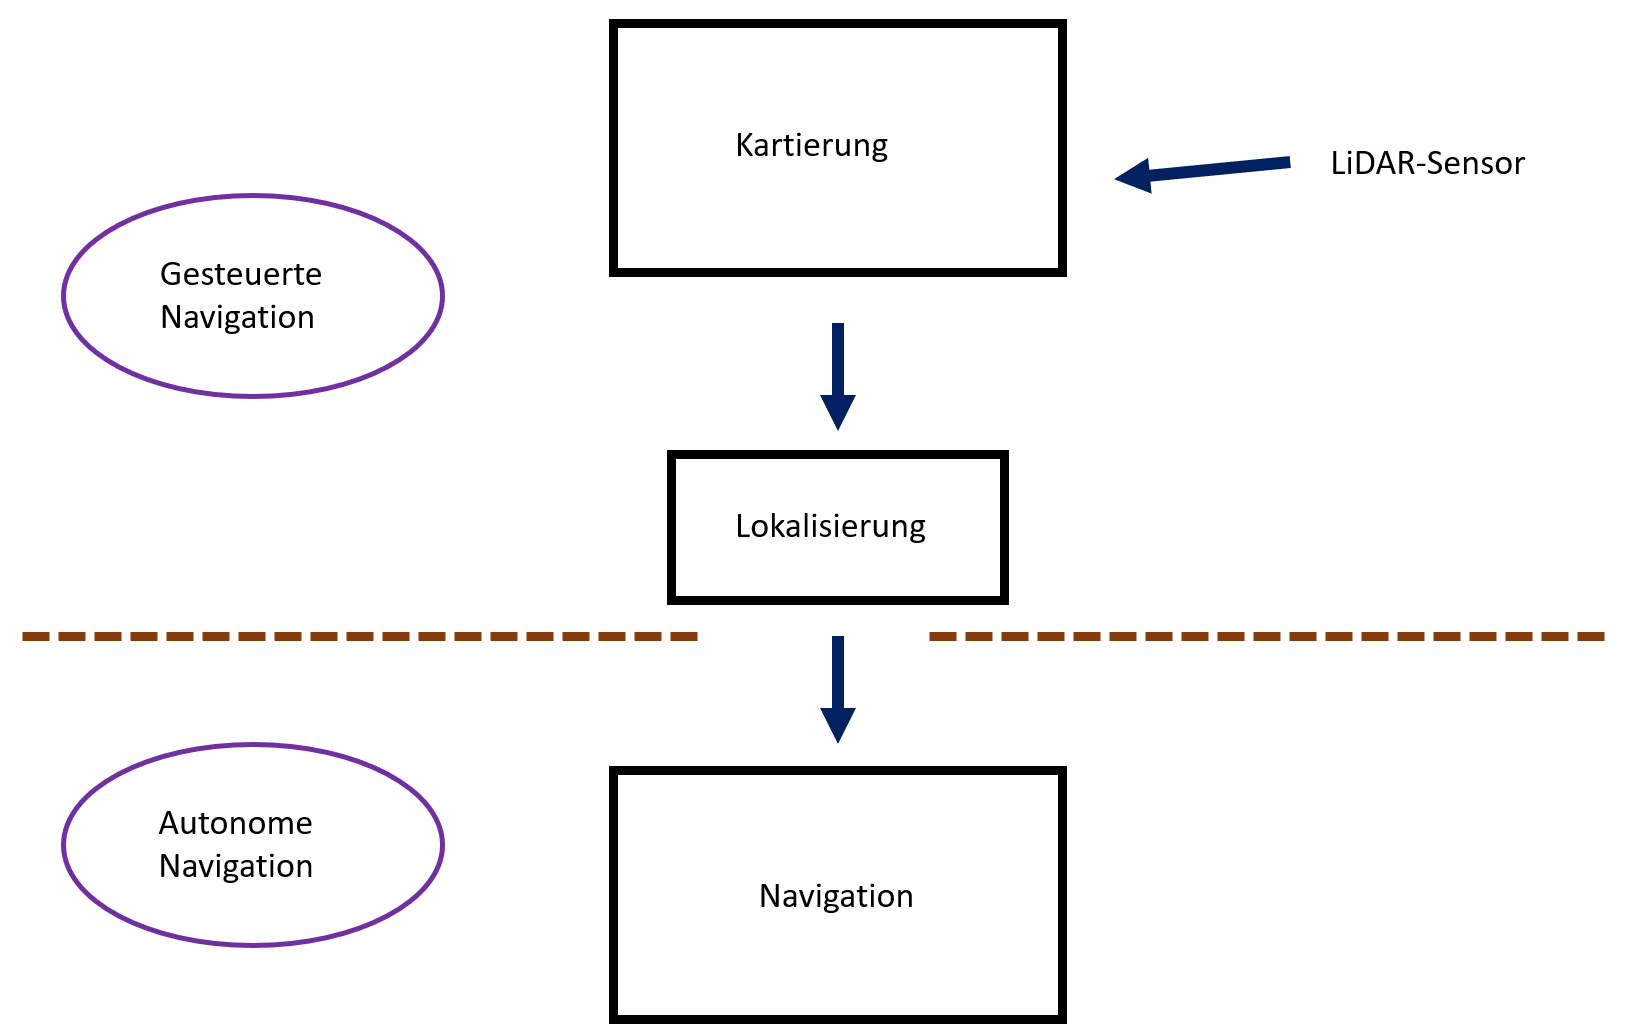
\includegraphics[height=8cm]{Bilder/overview_concept.png}
		\caption{Vorgehensweise zur autonomen Navigation} 
		\label{pic:overviewconcept}
	\end{figure}
Der Roboter wird anfangs mit Hilfe einer Tastatur oder eines Controllers gesteuert. Dabei wird, mit Hilfe des GMapping-Algorithmus, durch die Messdaten des LiDAR-Sensors, eine Karte der Umgebung erstellt. Damit der Karte nicht jedes mal erneut erstellen muss besteht auch die Möglichkeit, eine bereits existierende Karte einzulesen. Auf der erstellten Karte wird der Roboter lokalisiert und positioniert. Sind diese Bedingungen erfüllt, kann der Roboter durch ein Navigationspaket im Labyrinth navigieren, wobei keine Steuerung durch einen Menschen mehr benötigt wird.
}